\documentclass[reportComp]{thesis}
\usepackage[optidef,python,pseudo]{mypackage}

\title{模式识别作业六}
\school{数据科学与计算机学院}
\author{陈鸿峥}
\classname{17大数据与人工智能}
\stunum{17341015}
\headercontext{模式识别作业作业六}

\begin{document}

\maketitle

\begin{question}[\textsection 5 Q4]
考虑判别中用的超平面。
\begin{itemize}
\item [(a)] 证明在从超平面$g(\vx)=\vw^\T \vx+w_0 =0$到点$\vx_a$的距离为$|g(\vx_a)|/\norm{\vw}$,且对应的点是约束条件$g(\vx)=0$下的满足使$\norm{\vx-\vx_a}^2$最小的$\vx$。
\item [(b)] 证明$\vx_a$到超平面的投影为
\[\vx_p=\vx_a-\frac{g(\vx_a)}{\norm{\vw}^2}\vw\]
\end{itemize}
\end{question}
\begin{answer}
\begin{itemize}
	\item [(a)] 优化问题如下
	\begin{mini*}
		{\vx}{\norm{\vx-\vx_a}^2}{}{}
		\addConstraint{g(\vx)}{=\vw^\T \vx+w_0 =0}
	\end{mini*}
	构造拉格朗日函数(这里为方便计算,在约束项前面添加了常数$2$)
	\[\begin{aligned}f(\mathbf{x}, \lambda)&=\left\|\mathbf{x}-\mathbf{x}_{a}\right\|^{2}+2 \lambda[g(\mathbf{x})]\\
	&=\left\|\mathbf{x}-\mathbf{x}_{a}\right\|^{2}+2 \lambda\left[\mathbf{w}^\T  \mathbf{x}+w_{0}\right] \\
	&=\left(\mathbf{x}-\mathbf{x}_{a}\right)^\T \left(\mathbf{x}-\mathbf{x}_{a}\right)+2 \lambda\left(\mathbf{w}^\T  \mathbf{x}+w_{0}\right) \\
	&=\mathbf{x}^\T  \mathbf{x}-2 \mathbf{x}^\T  \mathbf{x}_{a}+\mathbf{x}_{a}^\T  \mathbf{x}_{a}+2 \lambda\left(\mathbf{x}^\T  \mathbf{w}+w_{0}\right)
	\end{aligned}\]
	分别求偏导有
	\[\begin{cases}
	{\frac{\partial f(\vx, \lambda)}{\partial \vx}=\vx-\vx_{a}+\lambda \vw=0} \\
	{\frac{\partial f(\vx, \lambda)}{\partial \lambda}=\vw^\T  \vx+w_{0}=0}
	\end{cases}\]
	联立可解得
	\[\lambda=\frac{\mathbf{w}^\T  \mathbf{x}_{a}+w_{0}}{\mathbf{w}^\T  \mathbf{w}}\]
	进而有
	\[\begin{aligned} \mathbf{x} &=\mathbf{x}_{a}-\lambda \mathbf{w} \\
	&=\left\{\begin{array}{ll}
	{\mathbf{x}_{a}-\left[\frac{\mathbf{w}^\T  \mathbf{x}_{a}+w_{0}}{\mathbf{w}^\T  \mathbf{w}}\right] \mathbf{w}} & { \mathbf{w} \neq \mathbf{0}} \\
	{\mathbf{x}_{a}} & { \mathbf{w}=\mathbf{0}}
	\end{array}
	\right.\end{aligned}\]
	代入原式得到距离最小值
	\[\begin{aligned}
	\left\|\mathbf{x}-\mathbf{x}_{a}\right\| &=\left\|\mathbf{x}_{a}-\left[\frac{\mathbf{w}^\T  \mathbf{x}_{a}+w_{0}}{\mathbf{w}^\T  \mathbf{w}}\right] \mathbf{w}-\mathbf{x}_{a}\right\| \\
	&=\left\|\left(\frac{\mathbf{w}^\T  \mathbf{x}_{a}+w_{0}}{\mathbf{w}^\T  \mathbf{w}}\right) \mathbf{w}\right\| \\
	&=\frac{\left|g\left(\mathbf{x}_{a}\right)\right|\|\mathbf{w}\|}{\|\mathbf{w}\|^{2}}=\frac{\left|g\left(\mathbf{x}_{a}\right)\right|}{\|\mathbf{w}\|}
	\end{aligned}\]
	符合题意
	\item [(b)] 由于(a)已经得到从超平面到$\vx$的最小距离,而$\vx_a$的投影即为拉格朗日求导等于零求出来的$\vx$值,即
	\[\begin{aligned}
	\mathbf{x}_{p} &=\mathbf{x}_{a}-\lambda \mathbf{w} \\
	&=\mathbf{x}_{a}-\frac{g\left(\mathbf{x}_{a}\right)}{\|\mathbf{w}\|^{2}} \mathbf{w}
	\end{aligned}\]
	其中
	\[\lambda=\frac{\mathbf{w}^\T  \mathbf{x}_{a}+w_{0}}{\mathbf{w}^\T  \mathbf{w}}=\frac{g\left(\mathbf{x}_{a}\right)}{\|\mathbf{w}\|^{2}}\]
\end{itemize}
\end{answer}

\begin{question}[\textsection 5 Q14]
考虑平方误差和准则函数(式(43))
\[J_s(\va)=\sum_{i=1}^n(\va^\T \vy_i-b_i)^2\]
令$b_i=b$,取如下6个训练点:
\begin{center}
\begin{tabular}{llll}
$\omega_1$&: $(1,5)^\T$  & $(2,9)^\T$  & $(-5,-3)^\T$ \\
$\omega_2$&: $(2,-3)^\T$  & $(-1,-4)^\T$  & $(0,2)^\T$ 
\end{tabular}
\end{center}
\begin{itemize}
	\item [(a)] 计算它的Hessian矩阵
	\item [(b)] 假定二次准则函数,计算最优学习率$\eta$
\end{itemize}
\end{question}
\begin{answer}
将训练集数据$\omega_1$和$\omega_2$构成矩阵,并扩增一个维度,得到
\[Y =\left(\begin{array}{rrr}{1} & {1} & {5} \\ {1} & {2} & {9} \\ {1} & {-5} & {-3} \\ {-1} & {-2} & {3} \\ {-1} & {1} & {4} \\ {-1} & {0} & {-2}\end{array}\right) \quad \mathbf{a}=\left(\begin{array}{r}{a_{1}} \\ {a_{2}} \\ {a_{3}}\end{array}\right) \quad \mathbf{b}=\left(\begin{array}{c}{b} \\ {b} \\ {b} \\ {b} \\ {b} \\ {b}\end{array}\right)\]
平方误差准则函数为
\[J_{s}(\mathbf{a})=\frac{1}{2} \sum_{i=1}^{n}\left(\mathbf{a}^\T  \mathbf{y}_{i}-b\right)^{2}=\frac{(Y  \mathbf{a}-\mathbf{b})^\T (Y  \mathbf{a}-\mathbf{b})}{2}\]
\begin{itemize}
	% 没有必要将一阶导求出具体值
	\item [(a)] 对准则函数求导得到
	\[\nabla J_{s}(\mathbf{a})=Y^\T (Y  \mathbf{a}-\mathbf{b})\]
	进而Hessian矩阵为
	\[H =\nabla^2 J_s(\va)=Y ^\T  Y =\left(\begin{array}{ccc}{6} & {-1} & {6} \\ {-1} & {35} & {36} \\ {6} & {36} & {144}\end{array}\right)\]
	\item [(b)] 由公式(14),最优学习率为
	\[\eta=\frac{\left[\nabla J_{s}(\mathbf{a})\right]^\T  \nabla J_{s}(\mathbf{a})}{\left[\nabla J_{s}(\mathbf{a})\right]^\T  H  \nabla J_{s}(\mathbf{a})}\]
	通过求解特征方程,得到$H$的特征值\footnote{特征值可通过$|H-\lambda I|=0$求解,这里则直接使用numpy指令np.linalg.eig进行计算。}为$5.417,24.57,155.0$,进而
	\[\frac{1}{\lambda_{\max}}=0.006452\leq\eta\leq 0.1846=\frac{1}{\lambda_{\min}}\]
\end{itemize}
\end{answer}

\begin{question}[\textsection 5 Q21]
证明MSE解法中的尺度因子$\alpha$和Fisher线性判别(5.8.2节)的对应关系为
\[\alpha=\left[1+\frac{n_{1} n_{2}}{n}\left(\mathbf{m}_{1}-\mathbf{m}_{2}\right)^\T  \mathbf{S}_{w}^{-1}\left(\mathbf{m}_{1}-\mathbf{m}_{2}\right)\right]^{-1}\]
\end{question}
\begin{answer}
% 推到前面的变换交代一下
由等式(54)有权重向量
\[\mathbf{w}=\alpha n \mathbf{S}_{w}^{-1}\left(\mathbf{m}_{1}-\mathbf{m}_{2}\right)\]
其中$\vw$满足
\[\left[\frac{1}{n} \mathbf{S}_{w}+\frac{n_{1} n_{2}}{n^{2}}\left(\mathbf{m}_{1}-\mathbf{m}_{2}\right)\left(\mathbf{m}_{1}-\mathbf{m}_{2}\right)^\T \right] \mathbf{w}=\mathbf{m}_{1}-\mathbf{m}_{2}\]

将$\vw$代入上式得到
\[\left[\frac{1}{n} \mathbf{S}_{w}+\frac{n_{1} n_{2}}{n^{2}}\left(\mathbf{m}_{1}-\mathbf{m}_{2}\right)\left(\mathbf{m}_{1}-\mathbf{m}_{2}\right)^\T \right] \alpha n \mathbf{S}_{w}^{-1}\left(\mathbf{m}_{1}-\mathbf{m}_{2}\right)=\mathbf{m}_{1}-\mathbf{m}_{2}\]
令
\[\theta=1+\frac{n_{1} n_{2}}{n^{2}}\left(\mathbf{m}_{1}-\mathbf{m}_{2}\right)^\T  \mathbf{S}_{w}^{-1}\left(\mathbf{m}_{1}-\mathbf{m}_{2}\right)\]
则
\[\alpha \theta\left(\mathbf{m}_{1}-\mathbf{m}_{2}\right)=\mathbf{m}_{1}-\mathbf{m}_{2}\]
由于这条等式对于所有$\vm_1$和$\vm_2$成立,因此我们有$\alpha\theta=1$,或者下式成立
\[\alpha=\left[1+\frac{n_{1} n_{2}}{n^{2}}\left(\mathbf{m}_{1}-\mathbf{m}_{2}\right)^\T  \mathbf{S}_{w}^{-1}\left(\mathbf{m}_{1}-\mathbf{m}_{2}\right)\right]^{-1}\]
\end{answer}

% 取消了!
\begin{question}[\textsection 5 Q28]
在5.10.2节给出的线性规划公式包含了一个极小化的人工变量$\tau$,且满足约束条件$\va^\T y_i+\tau>b_i$及$\tau\geq 0$。
证明得到的权向量使得以下准则函数极小化:
\[J_\tau(\va)=\max_{\va^\T \vy_i\leq b_i}[b_i-\va^\T \vy_i]\]
\end{question}
\begin{answer}
实际上即找
\[\forall i:\min \left\{t: t \geq 0, \mathbf{a}^\T  \mathbf{y}_{i}+t>b_{i}\right\}\]
而目标是使权重向量$\va$最小化准则函数
\[J_{t}(\mathbf{a})=\max _{i: \mathbf{a}^\T  \mathbf{y}_{i} \leq b_{i}}\left(b_{i}-\mathbf{a}^\T  \mathbf{y}_{i}\right)\]

将其分为线性可分和线性不可分两种情况处理。
\begin{itemize}
	\item [(a)] 线性可分情况下,存在$\va_o$使得$\va_o^\T \vy_i=b_i$,那么显然
	\[\forall t>0,i:\; \va_o^\T \vy_i+t > b_i\]
	因此我们有对于所有的$i$
	\[\begin{aligned}
	0 & \leq \min \left\{t: t \geq 0, \mathbf{a}^\T  \mathbf{y}_{i}+t>b_{i}\right\} \\
	 & \leq \min \left\{t: t \geq 0, \mathbf{a}^\T  \mathbf{y}_{i}+t>b_{i}\right\}=0
	\end{aligned}\]
	进而
	\[\min \left\{t: t \geq 0, \mathbf{a}^\T  \mathbf{y}_{i}+t>b_{i}\right\}=0\]
	得到的权重向量即为$\va_o$。
	由$J_t(\va)\geq 0,\forall\va$且$J_t(\va_o)=0$,可知
	\[\argmin_{\mathbf{a}} J_{t}(\mathbf{a})=\mathbf{a}_{o}\]
	这说明使$\va$最小化$J_t(\va)$等价于解决修改后的问题。
	\item [(b)] 线性不可分下,不存在$\va_o$使得$\va_o^\T \vy_i=b_i$,那么
	\[\begin{aligned}
	\forall i:\;\min _{t, \mathbf{a}}\left\{t: t \geq 0, \mathbf{a}^\T  \mathbf{y}_{i}+t>b_{i}\right\}
	&=\min _{t, \mathbf{a}}\left\{t: t \geq 0, t>b_{i}-\mathbf{a}^\T  \mathbf{y}_{i}\right\} \\
	&=\min _{t, \mathbf{a}}\left\{t: t \geq 0, t>\max _{i}\left(b_{i}-\mathbf{a}^\T  \mathbf{y}_{i}\right)\right\} \\
	&=\min _{t, \mathbf{a}}\left\{t: t>0, t>\max _{i}\left(b_{i}-\mathbf{a}^\T  \mathbf{y}_{i}\right)\right\} \\
	&=\min _{t, \mathbf{a}}\left\{t: t>\max _{i: \mathbf{a}^\T  \mathbf{y}_{i} \leq b_{i}}\left(b_{i}-\mathbf{a}^\T  \mathbf{y}_{i}\right)\right\} \\
	&=\min _{t, \mathbf{a}}\left\{\max _{i: \mathbf{a}^\T  \mathbf{y}_{i} \leq b_{i}}\left(b_{i}-\mathbf{a}^\T  \mathbf{y}_{i}\right)\right\} \\
	&=\min _{\mathbf{a}} J_{t}(\mathbf{a})
	\end{aligned}\]
\end{itemize}
\end{answer}

\begin{question}[\textsection 5 Q32]
考虑支持向量机和分属两类的训练样本:
\begin{center}
\begin{tabular}{llll}
$\omega_1$: & $(1,1)^\T$  & $(2,2)^\T$  & $(2,0)^\T$ \\
$\omega_2$: & $(0,0)^\T$  & $(1,0)^\T$  & $(0,1)^\T$ 
\end{tabular}
\end{center}
\begin{itemize}
	\item [(a)] 在图中作出这6个训练点,构造具有最优超平面和最优间隔的权向量。
	\item [(b)] 哪些是支持向量?
	\item [(c)] 通过寻找拉格朗日待定系数$\alpha_i$来构造在对偶空间的解,并将它与(a)中的结果比较。
\end{itemize}
\end{question}
\begin{answer}
\begin{itemize}
	\item [(a)] 按序编号
	\[\begin{aligned}
	\omega_{1}&: \mathbf{x}_{1}=\left(\begin{array}{c}{1} \\ {1}\end{array}\right), \mathbf{x}_{2}=\left(\begin{array}{l}{2} \\ {2}\end{array}\right), \mathbf{x}_{3}=\left(\begin{array}{l}{2} \\ {0}\end{array}\right)\\
	\omega_{2}&:\mathbf{x}_{4}=\left(\begin{array}{l}{0} \\ {0}\end{array}\right), \mathbf{x}_{5}=\left(\begin{array}{l}{1} \\ {0}\end{array}\right), \mathbf{x}_{6}=\left(\begin{array}{l}{0} \\ {1}\end{array}\right)
	\end{aligned}\]
	且$z_1=z_2=z_3=-1,z_4=z_5=z_6=1$。
	如下图所示,考虑做恒等映射$\vy_k=\varphi(\vx_k)=\vx_k$,则在$\vy$空间上最优超平面为$y_1+y_2=3/2$,即
	\[(3 / 2,-1,-1)^\T \left(1,y_{1},y_{2}\right)=0\]
	将其做放缩变换($\times 2$),得到权向量为$(3,-2,-2)^\T $。

	\begin{figure}[H]
	\centering
	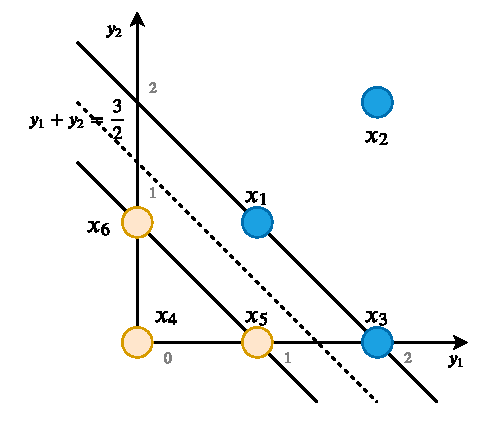
\includegraphics[width=0.5\linewidth]{fig/Q32.pdf}
	\end{figure}
	最优间隔为从样本点到超平面的最小距离为$1/2\sin(\pi/4)=\sqrt{2}/4$。
	\item [(b)] 从上图可以清晰看出,支持向量为
	\[\left\{\mathbf{x}_{1}, \mathbf{x}_{3}, \mathbf{x}_{5}, \mathbf{x}_{6}\right\}=\left\{(1,1)^\T ,(2,0)^\T ,(1,0)^\T ,(0,1)^\T \right\}\]
	\item [(c)] 最大化式(109)给出的准则函数
	\[\begin{aligned}
	& L(\boldsymbol{\alpha})=\sum_{k=1}^{n} \alpha_{k}-\frac{1}{2} \sum_{k, j}^{n} \alpha_{k} \alpha_{j} z_{k} z_{j} \mathbf{y}_{j}^\T  \mathbf{y}_{k}\\
	& \text{s.t.} \sum_{k=1}^{n} z_{k} \alpha_{k}=0,\;\alpha_k\geq 0
	\end{aligned}\]
	使用约束条件,可用下式消除一个元
	\[\alpha_{6}=\alpha_{1}+\alpha_{2}+\alpha_{3}-\alpha_{4}-\alpha_{5}\]
	求偏导得到
	\[\left[\begin{array}{ccccc}{-1} & {-2} & {-2} & {0} & {1} \\ {-2} & {-5} & {2} & {-1} & {1} \\ {-2} & {2} & {-5} & {1} & {1} \\ {0} & {-1} & {1} & {-1} & {-1} \\ {1} & {1} & {3} & {-1} & {-2}\end{array}\right]\left[\begin{array}{c}{\alpha_{1}} \\ {\alpha_{2}} \\ {\alpha_{3}} \\ {\alpha_{4}} \\ {\alpha_{5}}\end{array}\right]=\left[\begin{array}{c}{-2} \\ {-2} \\ {-2} \\ {0} \\ {0}\end{array}\right]\]
	但是这个方程组不相容,因此最大值一定在边界处取到(即有些$\alpha_i$消失了)。
	接下来尝试分别令每一个$\alpha_i=0$来求解。
	\begin{itemize}
	\item $\alpha_1=0$时,
	\[\frac{\partial L\left(0, \alpha_{2}, \alpha_{3}, \alpha_{4}, \alpha_{5}\right)}{\partial \alpha_{i}}=0\]
	可解得$\boldsymbol{\alpha}=(0,-1/10,-1/10,8/5,-8/5,-4/5)^\T $
	\item $\alpha_2=0$时,下式导致不相容
	\[\frac{\partial L\left(\alpha_{1}, 0, \alpha_{3}, \alpha_{4}, \alpha_{5}\right)}{\partial \alpha_{i}}=0\]
	\item $\alpha_3=0$时,下式导致不相容
	\[\frac{\partial L\left(\alpha_{1}, \alpha_{2}, 0, \alpha_{4}, \alpha_{5}\right)}{\partial \alpha_{i}}=0\]
	\item $\alpha_4=0$时,
	\[\frac{\partial L\left(\alpha_{1}, \alpha_{2}, \alpha_{3}, 0, \alpha_{5}\right)}{\partial \alpha_{i}}=0\]
	解得$\boldsymbol{\alpha}=1/5(16,0,4,0,14,6)^\T $,满足$\alpha_i\geq 0$的限制,此时准则函数$L(\valpha)=4$
	\item $\alpha_5=0$时,
	\[\frac{\partial L\left(\alpha_{1}, \alpha_{2}, \alpha_{3}, \alpha_{4}, 0\right)}{\partial \alpha_{i}}=0\]
	得到$\valpha=1 / 5(2,2,2,0,0,6)^\T $,满足$\alpha_i\geq 0$的限制,此时准则函数$L(\valpha)=1.2$
	\end{itemize}
	故$\boldsymbol{\alpha}=1/5(16,0,4,0,14,6)^\T $时,准则函数$L$取得最大值,且满足限制条件。

	接下来计算权向量$\va$。
	视$\va$为变量,尝试最小化式(108)中的
	\[L(\mathbf{a}, \boldsymbol{\alpha})=\frac{1}{2}\|\mathbf{a}\|^{2}-\sum_{k=1}^{n} \alpha_{k}\left[z_{k} \mathbf{a}^\T  \mathbf{y}_{k}-1\right]\]
	求导有
	\[\frac{\partial L}{\partial \mathbf{a}}=\mathbf{a}-\sum_{k=1}^{n} \alpha_{k} z_{k} \mathbf{y}_{k}=\mathbf{0}\]
	进而$\va=(0,-2,-2)^\T $。

	最后确定$a_0$。
	使用支持向量$\vy=(1,1,1)^\T $,满足$\va^\T \vy_1z_1=1$,得到
	\[-\left(\begin{array}{c}{a_0} \\ {-2} \\ {-2}\end{array}\right)(1,1,1)=-a_{0}+4=1\]
	求得$a_0=3$,最终的权向量为$\va=(3,-2,-2)^\T $。
\end{itemize}
\end{answer}

\end{document}